\documentclass{article}
\usepackage{graphicx} % Required for inserting images
\usepackage{float}
\usepackage[T1]{fontenc}
\usepackage{amsmath}
\usepackage[margin=1in]{geometry}
\usepackage{booktabs}
\usepackage{tabularx}
\usepackage[hidelinks]{hyperref}

\title{Stop levels and an earlier profit-take on the SPY gamma book}
\author{Experiment report \textperiodcentered{} L/S Gamma Desk, QUANTT}
\date{2026-10-16}

\begin{document}

\maketitle

\textbf{Question:} Do tighter stops (short stop at 0.5x credit, long stop at 0.25x premium) cut the daily 5\% expected shortfall of the book by at least 20\% at a small cost in P\&L (H1)? Does taking profit on shorts at 25\% of the credit instead of 50\% raise net P\&L without a worse tail (H2)?

\textbf{Method:} Pre-registered backtest (hypothesis card committed before any run). The live paper rules (\texttt{configs/\allowbreak{}paper.\allowbreak{}toml}) are replayed on R2 replay snapshots v1 (config\_hash b040760187f0) over the development window 2014-06-02 to 2024-12-31. The hold-out (2025-01-01 to 2026-07-10) was not used. Three variants change only \texttt{[exit]}: \texttt{tight} (short\_stop\_mult 0.5, long\_stop\_frac 0.25; primary for H1), \texttt{profit25} (short\_profit\_frac 0.25; H2) and \texttt{both} (all three; reported only). The stop cool-off stays at the live 1 day. Each variant ran once at 1x and 2x spreads and is compared with baseline trial 1 at the same spread multiple. Costs are \$0.65 per contract and \$0.005 per share, with a \$1 minimum per order. Exits are checked once a day at 10:15 ET, as live.

\begin{quote}This report was written by Claude at the PM's request.\end{quote}

\section{Result vs the pass bar}

Every check had to hold at both 1x and 2x. ES size is the absolute value of the daily 5\% expected shortfall in USD; P\&L is net USD for one contract.

\textbf{H1 (tight): failed.} The tail did not shrink; it got slightly worse in both halves and at both spread levels.

\begin{center}\small
\begin{tabularx}{\linewidth}{>{\raggedright\arraybackslash}X l l l l l}
\toprule
\textbf{Check} & \textbf{1x value} & \textbf{1x bar} & \textbf{2x value} & \textbf{2x bar} & \textbf{Result} \\
\midrule
ES size, full window & 98.1 & \ensuremath{\leq} 77.2 & 107.1 & \ensuremath{\leq} 83.6 & fail \\
ES size, 2014-06..2019-12 & 49.0 & < 47.9 & 55.8 & < 53.2 & fail \\
ES size, 2020-01..2024-12 & 134.1 & < 132.9 & 144.4 & < 142.9 & fail \\
Net P\&L, full window & \ensuremath{-}2,330.7 & \ensuremath{\geq} \ensuremath{-}2,359.5 & \ensuremath{-}4,540.3 & \ensuremath{\geq} \ensuremath{-}4,422.3 & fail (2x) \\
\bottomrule
\end{tabularx}
\end{center}

\textbf{H2 (profit25): failed.} It helped in the first half but lost more in the second half, so full-window net P\&L was below baseline at both spreads. The tail was unchanged.

\begin{center}\small
\begin{tabularx}{\linewidth}{>{\raggedright\arraybackslash}X l l l l l}
\toprule
\textbf{Check} & \textbf{1x value} & \textbf{1x bar} & \textbf{2x value} & \textbf{2x bar} & \textbf{Result} \\
\midrule
Net P\&L, full window & \ensuremath{-}2,153.4 & > \ensuremath{-}2,059.5 & \ensuremath{-}4,170.8 & > \ensuremath{-}4,122.3 & fail \\
Net P\&L, 2014-06..2019-12 & \ensuremath{-}922.2 & > \ensuremath{-}986.2 & \ensuremath{-}1,450.7 & > \ensuremath{-}1,511.3 & pass \\
Net P\&L, 2020-01..2024-12 & \ensuremath{-}1,231.2 & > \ensuremath{-}1,073.3 & \ensuremath{-}2,720.1 & > \ensuremath{-}2,610.9 & fail \\
ES size, full window & 96.6 & \ensuremath{\leq} 106.1 & 104.5 & \ensuremath{\leq} 115.0 & pass \\
\bottomrule
\end{tabularx}
\end{center}

\subsection{Full-window summary (no bar for \texttt{both})}

\begin{center}\small
\begin{tabularx}{\linewidth}{l l l l l l >{\raggedright\arraybackslash}X}
\toprule
\textbf{Variant} & \textbf{Spread} & \textbf{Net P\&L} & \textbf{Sharpe} & \textbf{Max DD} & \textbf{ES 5\%} & \textbf{Trades} \\
\midrule
baseline & 1x & \ensuremath{-}2,059.5 & \ensuremath{-}0.356 & 3,027 & \ensuremath{-}96.5 & 131 \\
tight & 1x & \ensuremath{-}2,330.7 & \ensuremath{-}0.398 & 3,027 & \ensuremath{-}98.1 & 133 \\
profit25 & 1x & \ensuremath{-}2,153.4 & \ensuremath{-}0.373 & 3,017 & \ensuremath{-}96.6 & 132 \\
both & 1x & \ensuremath{-}2,555.9 & \ensuremath{-}0.439 & 3,017 & \ensuremath{-}98.2 & 134 \\
baseline & 2x & \ensuremath{-}4,122.3 & \ensuremath{-}0.681 & 4,258 & \ensuremath{-}104.5 & 131 \\
tight & 2x & \ensuremath{-}4,540.3 & \ensuremath{-}0.732 & 4,676 & \ensuremath{-}107.1 & 133 \\
profit25 & 2x & \ensuremath{-}4,170.8 & \ensuremath{-}0.691 & 4,315 & \ensuremath{-}104.5 & 132 \\
both & 2x & \ensuremath{-}4,722.7 & \ensuremath{-}0.765 & 4,867 & \ensuremath{-}107.1 & 134 \\
\bottomrule
\end{tabularx}
\end{center}

\section{Charts}

\begin{figure}[H]\centering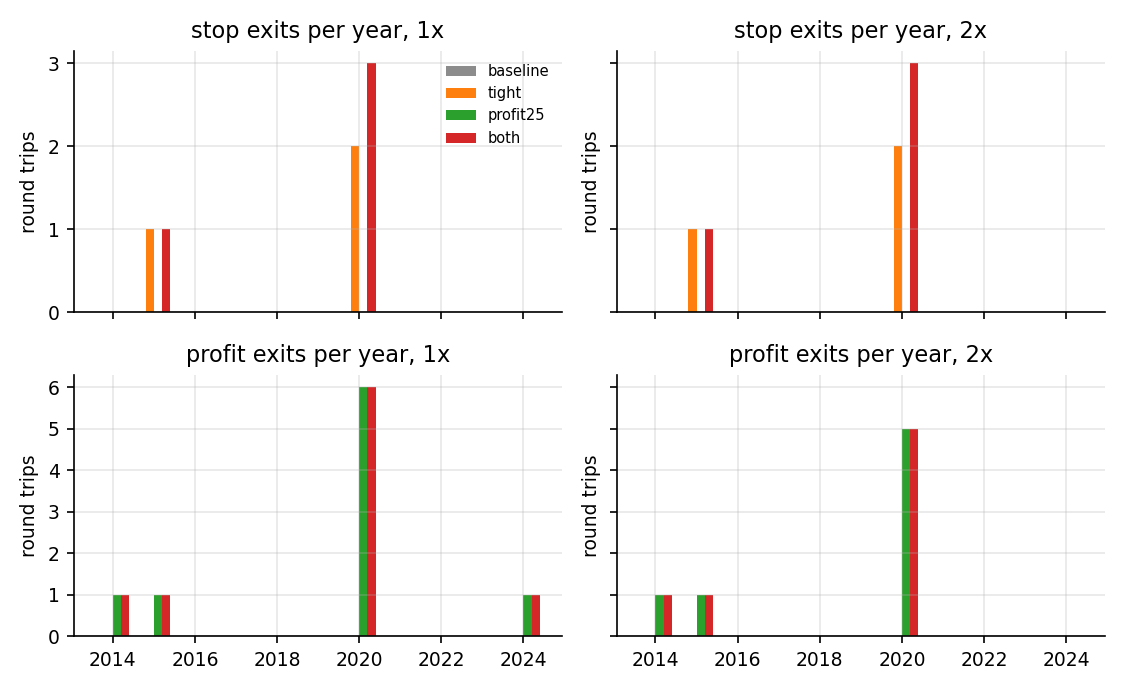
\includegraphics[width=0.92\linewidth]{figures/exits_per_year.png}\caption{Stop and profit exits per year, by variant, at 1x and 2x spreads}\end{figure}

The tighter stops fired only 3 times in ten and a half years: one in 2015 and two in the 2020 sell-off, at both spread levels (two shorts and one long). The 25\% profit-take fired 9 times at 1x and 7 at 2x, mostly in 2020. The baseline never stopped or took profit. With so few events, every result below rests on a handful of positions.

\begin{figure}[H]\centering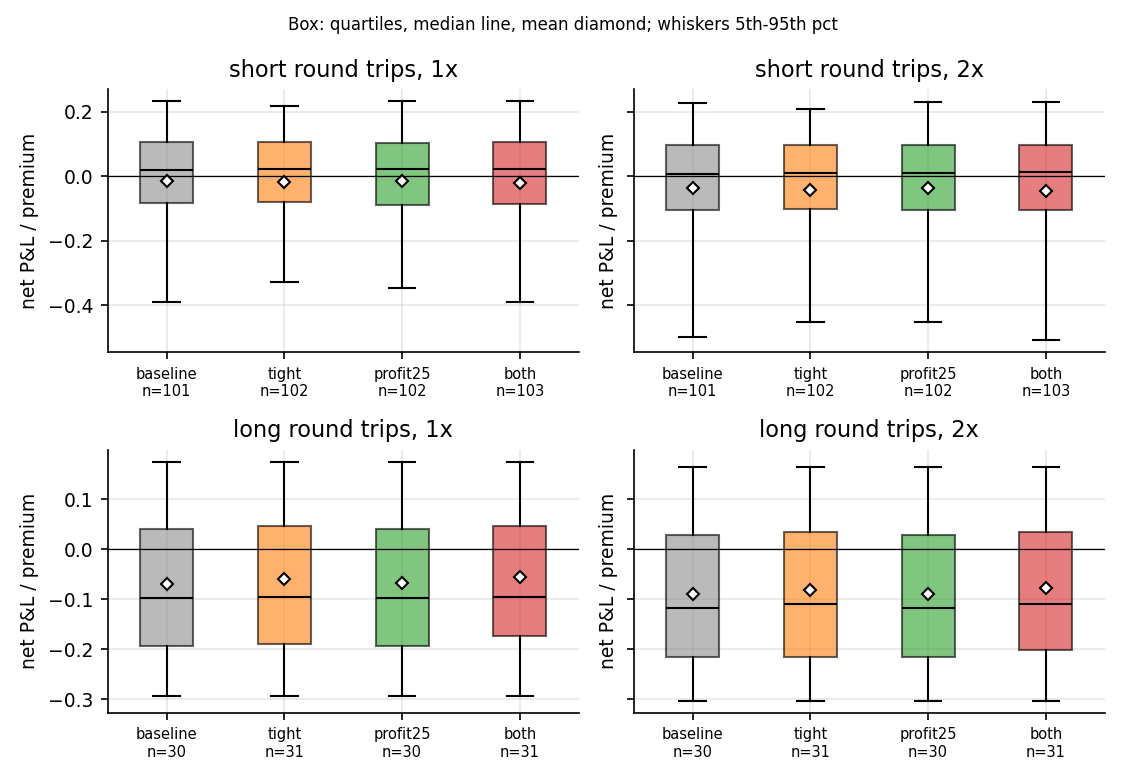
\includegraphics[width=0.92\linewidth]{figures/pnl_premium.png}\caption{Net P\&L of round trips as a multiple of premium, short and long, by variant. Box: quartiles; whiskers: 5th to 95th percentile}\end{figure}

The distributions are nearly the same across variants. At 1x the 5th percentile of short round trips is about \ensuremath{-}0.39x premium for the baseline, \texttt{tight} and \texttt{profit25} alike (\ensuremath{-}0.44x for \texttt{both}). The whiskers sit on single trades, so their small shifts mean little. The worst short under \texttt{tight} is worse than the baseline's (\ensuremath{-}1.27x against \ensuremath{-}0.78x premium): it is the 2015-08-24 stop, which closed after the move. Long round trips are almost identical, because only one long was stopped.

\begin{figure}[H]\centering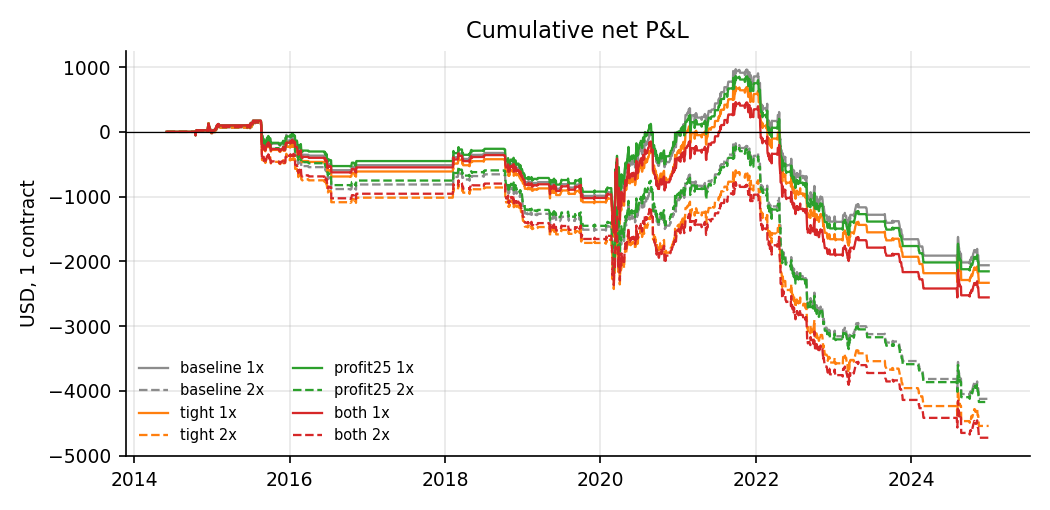
\includegraphics[width=0.92\linewidth]{figures/cum_pnl.png}\caption{Cumulative net P\&L, 1x (solid) and 2x (dashed)}\end{figure}

All four curves follow the baseline closely. They separate in two places: August 2015 and the 2020 sell-off, when the stops fired. In both, the stopped variants end up lower. \texttt{profit25} runs slightly above the baseline until 2020 and slightly below it afterwards.

\begin{figure}[H]\centering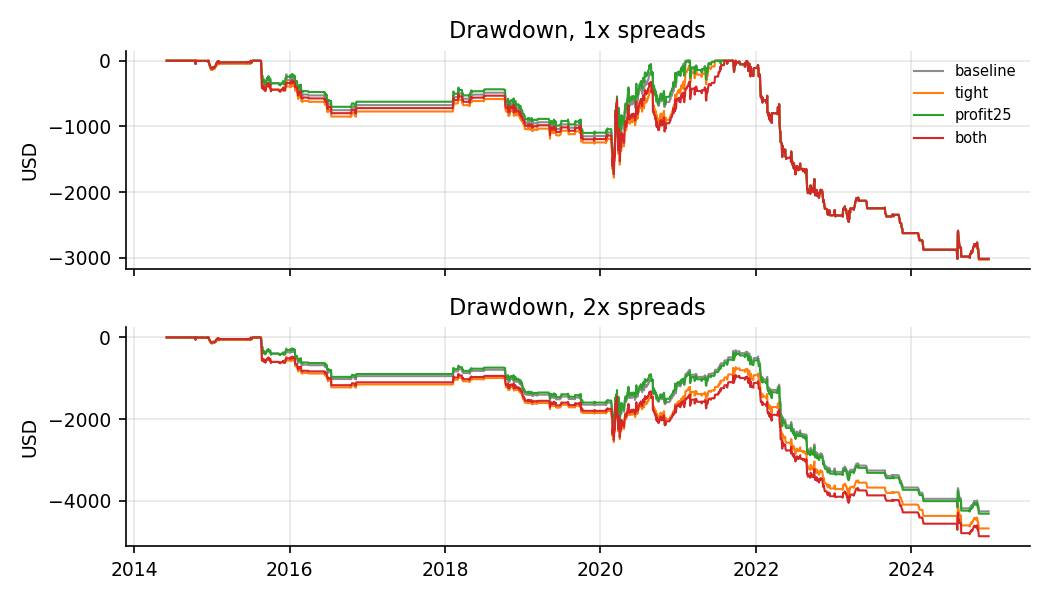
\includegraphics[width=0.92\linewidth]{figures/drawdown.png}\caption{Drawdown from the running peak, 1x and 2x}\end{figure}

The 1x maximum drawdown is the 2022-2024 slide for every variant (\$3,017 to \$3,027). The small gap comes from one profit-take on 2024-10-24 in \texttt{profit25} and \texttt{both}, which moved their trough to 2024-08-05. At 2x, \texttt{tight} and \texttt{both} start that slide from a lower level, so their maximum drawdown is \$400 to \$600 larger.

\begin{figure}[H]\centering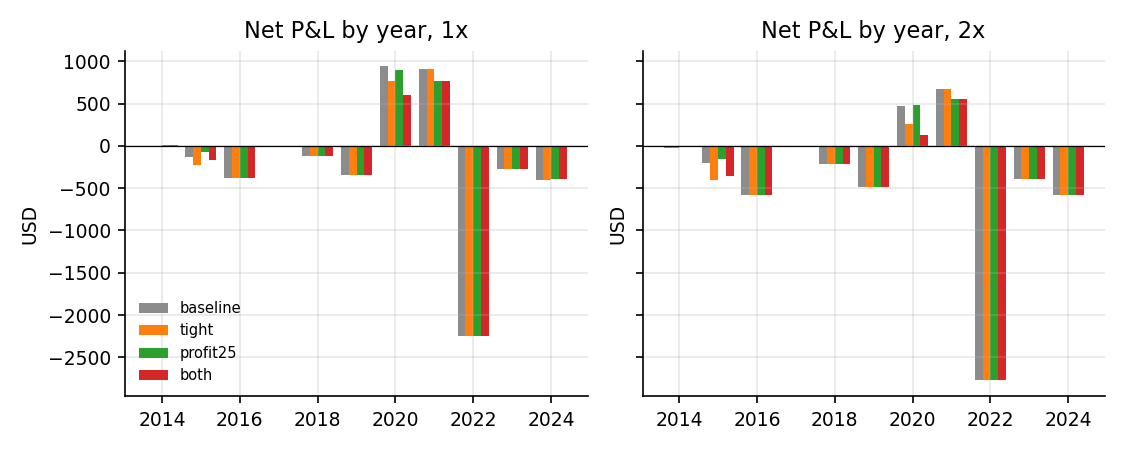
\includegraphics[width=0.92\linewidth]{figures/yearly.png}\caption{Net P\&L by year, 1x and 2x}\end{figure}

The yearly bars differ mainly in 2015, 2020 and 2021 (\texttt{profit25} and \texttt{both} also differ by about \$10 in 2014 and 2024). The large 2022 loss is the same for every variant: no exit rule touched it, because no position in 2022 reached the stop levels at the 10:15 check.

\begin{figure}[H]\centering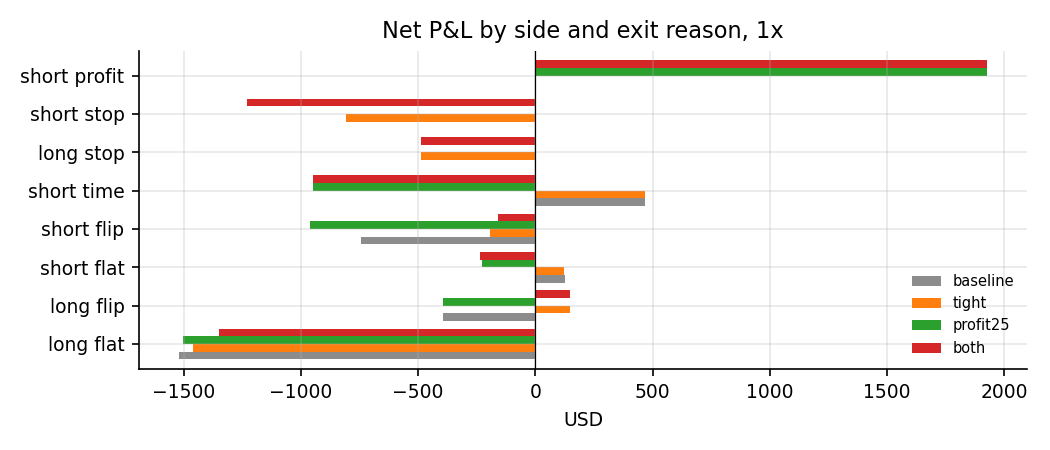
\includegraphics[width=0.92\linewidth]{figures/by_reason.png}\caption{Net P\&L by side and exit reason, 1x}\end{figure}

The 3 stopped positions lost \$1,297 net at 1x. In the baseline, the same 3 positions stayed open and closed on a flip signal for a loss of \$924, so the stop locked in losses that later partly recovered. The profit-take works the other way: at 1x, 8 of its 9 positions also exist in the baseline, and on those it earned \$254 more than the baseline did, mostly by closing winners before expiry. That gain was more than offset by the shorts opened afterwards. The short time-exit bucket swings from +\$470 to \ensuremath{-}\$948, mainly in 2020 to 2021.

\begin{figure}[H]\centering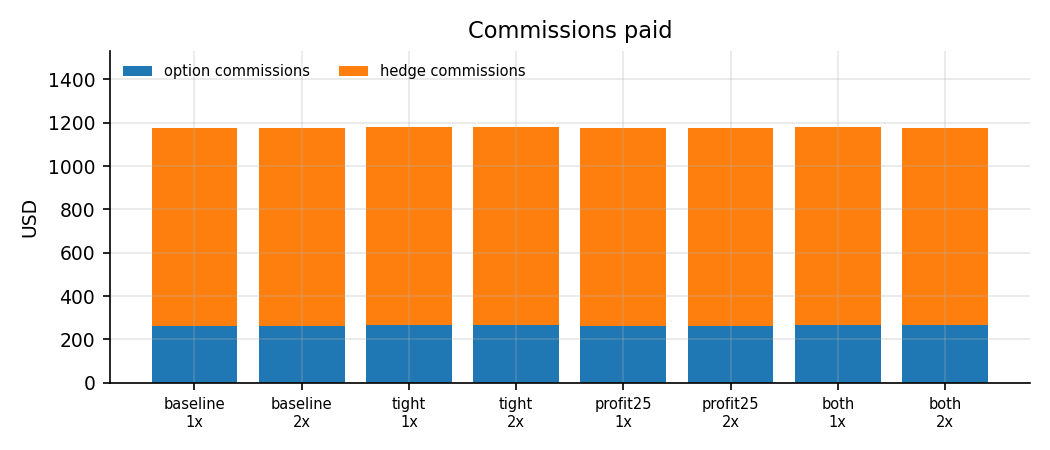
\includegraphics[width=0.92\linewidth]{figures/fees.png}\caption{Commissions paid, by variant and spread}\end{figure}

Commissions are the same for every variant (about \$1,175, of which \$910 to \$914 is hedge orders at the \$1 minimum). Fees don't explain the differences.

\section{Analysis}

The stops can't cut daily expected shortfall because of how they are checked. The worst 5\% of days are 129 days in every run, and 127 of the 129 are the same days in \texttt{tight} and the baseline. The worst single day (\ensuremath{-}\$468) is the same in all four variants. A stop checked once a day at 10:15 acts only after the move that triggers it. It can't stop the gap day that makes up the tail; it only closes the position the next morning. In this sample the baseline positions mostly recovered after such days: the worst short only reached \ensuremath{-}0.78x credit. Closing them at that point turned temporary losses into realized ones and slightly worsened both the tail and the P\&L. The 20\% ES cut that H1 needed would require removing losses on the tail days themselves, which a daily per-position stop can't do.

The 25\% profit-take did what it promised on the trades it closed. Those positions were worth more when closed early than when held, and the first half (2014-2019) beat the baseline at both spreads. But closing a short early frees the book to open the next short, and in 2020-2021 those follow-on shorts lost more than the early exits had gained. That follow-on effect is a path effect from a few events (7 to 9 profit-takes), so the half-by-half result is close to noise. The pre-registered bar asked for a gain in both halves and over the full window, and it got neither the second half nor the full window.

\texttt{both} combines the two weaknesses: it is the worst variant at both spreads.

\section{Verdict}

\textbf{H1 failed, H2 failed.} The tighter stops made the daily tail slightly worse instead of cutting it by 20\%, and at 2x spreads they also cost more than \$300. The 25\% profit-take lost to the baseline over the full window and in 2020-2024 at both spreads, although its tail was unchanged and it beat the baseline in 2014-2019. Neither change should go to \texttt{configs/\allowbreak{}paper.\allowbreak{}toml}. No hold-out run is needed.

\section{Caveats}

\begin{itemize}

\item \textbf{In-sample idea.} The idea for this experiment came from the baseline on the same window (no stop or profit-take ever fired there), so even a pass would only have been in-sample evidence.

\item \textbf{Very few events.} 3 stops and 7 to 9 profit-takes in ten and a half years. The differences come from 2015, 2020-2021 and one profit-take in 2024.

\item \textbf{Daily checks only.} Exits are checked once a day at 10:15, as in live trading. An intraday stop could behave differently. The replay snapshots support checks every 30 minutes (extra \texttt{[schedule] hedge} times, with spot implied from put-call parity), but that was not tested here.

\item \textbf{One contract.} The \$1 minimum per order is large relative to the position size (hedge commissions are about 78\% of all fees).

\item \textbf{Spread model.} It was fitted on about two weeks of calm 2026 live quotes; the 2x run is the stress check.

\item \textbf{Missing days.} Month-end R2 days are missing; 3.3\% of scheduled times were skipped in every run.

\end{itemize}

\section{Trials}

This experiment registered 6 trials (3 variants at 1x and 2x, from one run of \texttt{experiment.\allowbreak{}py}), plus the baseline's 2, for 8 in total. The baseline regression check that reproduced trial 1 was not registered. \texttt{tight} has exactly the same config as \texttt{cool1} in the parallel experiment 2026-10-16-stop-cooloff (0.5x credit, 0.25x premium, 1-day cool-off). The two gave identical numbers: all registry metrics, daily P\&L and trade P\&L match at 1x and 2x. The same test is therefore registered twice (4 trials) across the desk. The charts were rebuilt once with \texttt{-\allowbreak{}-\allowbreak{}report-\allowbreak{}only} to fix an axis; that reads saved runs and adds no trial.

\end{document}
